\documentclass[10pt,conference,compsocconf]{IEEEtran}

\usepackage{hyperref}
\usepackage{graphicx}	% For figure environment
\usepackage{amsmath}
\usepackage{placeins}

\begin{document}
\title{ML Project 2 - Report}

\author{
  Sarah Mikami, Samuel Waridel and Florian Kolly \\
  \textit{CS433, EPFL 2024}
  \textit{ML4Science project | TNE Laboratory}
}

\maketitle

\begin{abstract}

\end{abstract}

\section{Introduction}
Machine Learning (ML) is has become a central tool in neuroscience, with applications in neural engineering (e.g. Brain-Computer Interfaces, BCIs), diagnostics and fundamental research. For instance, Jalilifard et al. \cite{EmotionClassificationSVM} demonstrated the efficacy of Support Vector Machine (SVM) classifiers in basic emotions recognition, while Bose et al. \cite{EEGRandomForset} used Random Forest classifiers to automate seizure detection in epileptic patients with high accuracy. Indeed, all major ML methods have been applied to neural signals classification\cite{EEGMLReview}.

In this work, we examine the applications of such ML techniques in three classification problems using sEEG signals: i) distinguishing between the execution and observation of a movement; ii) differentiating between grasping a small versus a large object; iii) differentiating between observing the grasp of a small versus a large object.

Section \ref{sec:problem} outlines the data acquisition process and its relevance to our classification tasks. In Section \ref{sec:analysis}, we describe the preprocessing of the sEEG signals and the extraction of relevant features. Sections \ref{sec:actionrecognition} and \ref{sec:objectrecognition} present the models applied to our classification problems and their performance. In Section \ref{sec:deeplearning}, we explore the idea of using only Deep Learning (DL) to directly extract features from the EEG signal. Finally, we discuss our results in Section \ref{sec:discussion} and conclude in Section \ref{sec:conclusion}.

\section{Data acquisition and problem specification}
\label{sec:problem}
The dataset comprises signals recorded from four participants, each implanted with sEEG electrodes in distinct brain regions. During multiple experimental sessions, participants were instructed to either observe or execute specific motor tasks. These tasks involved two types of movements: a palmar grasp (force-based movement) and a pinch grasp (precision-based movement). Each session included multiple trials structured as follows: in an execution trial, the trial begins with a start cue. One second later, a light cue signals the type of object (small or large) to be targeted. This light remains illuminated for 0.5 seconds before turning off. After an additional 1.5 seconds, a "go" signal prompts the participant to lift their hand from the resting position, grasp the indicated object, return it to its original location, and place their hand back in the resting position. Observation trials followed an identical structure, except that participants passively observed the experimenter performing the actions. A light cue indicated the participant's role (execution or observation) in each trial.

\begin{figure}[h!]
  \center
  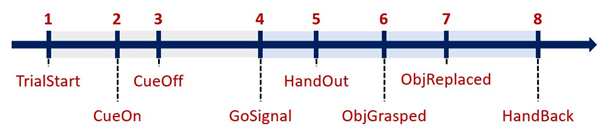
\includegraphics[width=\linewidth]{images/2024-12-11-13-41-48.png}
  \caption{Timing of the trials}
\end{figure}
\FloatBarrier

\section{Data analysis}
\label{sec:analysis}
In this section, we describe the preprocessing and analysis of the data. The dataset is a dictionary containing four subjects. Each subject participated to a number of sessions, ranging from only one session (subjects s6 and s7) up to three (subject s11). During each sessions, the subjects completed 256 tasks, equally distributed as observation or execution tasks. The channels are not identical across subjects.

\subsection{Channel responsiveness}
We first filtered the channels of interest: for a given channel and task, we define i) the \textit{baseline signal} as the average signal of all trials corresponding to the task in the one second between the start of the trial (1) and the cue light turning on (2), ii) the \textit{effect signal} as the average signal of all trials corresponding to the task in the one second around the instant at which the object is grasped (6) (either by the subject, or the experimenter). Using Welch's method\cite{welch}, we compute the power spectral density (PSD) for both the \textit{baseline signal} and the \textit{effect signal}. We then compare the PSDs of those signals in a t-test and define a \textit{responsive channel} as a channel with a statistically significative t-test (\(\alpha<0.05\)). This step is done simultaneously for channels that are responsive only in the observation trials, channels that are responsive only in the execution trials, and channels that are responsive for both types. As the channels are not identical across subjects, the results are specific to a single subject, so the preprocessing has to be done subject-wise.

\subsection{Data preprocessing}
The signals (one signal per channel) of each trial is preprocessed in three steps.
\begin{enumerate}
  \item Subsampling: the signal is subsampled from 2048Hz to 500Hz to reduce the computation needs. As our EEG data contains information up to around 150Hz, this subsampling respect the Nyquist criterion.
  \item Z-score correction: Each EEG signal is normalized with Z-score normalization using the mean and standard deviation of the \textit{baseline signal}
  \item Resampling: finally, we resample our trials such that all have the same number of timepoints
\end{enumerate}

\subsection{Feature extraction}
TODO

\begin{itemize}
    \item Amplitude, shape of response \(\to\) difference?
    \item Response pattern at the same timing?
    \item Similar frequency characteristics?
    \item Correlation? High correlation suggests congruence
    \item Are the results obtained similar for both movements?
\end{itemize}

\section{Action recognition}
\label{sec:actionrecognition}
In this first classification task, we train and optimize different family of ML models to predict whether the participant was executing the movement, or observing it. We use only channels that are responsive to both movements. Due to the very different tasks compared here, we expect all our models to perform quite well.

\subsection{Relevant channels}
Which regions have the most responsive channels?

\begin{itemize}
    \item Across participant: same region? same nb of responsive channels?
    \item Do we find the expected regions? Link to mvt execution / observation?
\end{itemize}

For channels where we have response for both ex \& obs, are the responses congruent (similar pattern) or incongruent (different)?

\subsection{Models}
\paragraph{Logistic regression}
Logistic regression (LR) is a computationally simple ML technique, and has previously used in EEG classification\cite{SUBASI200587, NIPS2006_35937e34}. Here, we use LR to create two different baselines on which to compare more complex models. Firstly, we selected non-responsive channels and extracted features from them. This first baseline, which we expect to work only slightly above chance, serves as a confirmation that our channel selection is indeed a valuable initial preprocessing step. A second baseline is to train another LR model on the features extract from the responsive channel. It is the performance of this model on which we will compare all other models. We also applied PCA to reduce the dimension of our data to create a third LR model. Every time PCA is applied, we keep 95\% of the explained variance.

\paragraph{SVM}
We train two Singular Vector Machines (SVM) models, with and without PCA. SVM can handle high dimensional data, even for small datasets. Although more computationally than other methods, it is widely used in EEG classification with good results \cite{knn_svm_review}.

\paragraph{Random forest}
Random Forest (RF) classifiers combine the output of multiple decision trees to reach a single result. Decision trees are algorithms classify data by creating branches depending on the value of a feature: at the end of all the branches, the leaves provide a classification result. As decision trees are prone to errors and overfitting, it is recommended to combine multiple decision trees together to improve the accuracy. A RF classifier do exactly that, by adding additional constraints to make sure the trees are different.

\paragraph{MLP}
In addition to traditional ML models, we also train Multilayer Perceptron (MLP). We chose to include MLP as it is widely used in EEG classification\footnote{3'610 results for 'EEG MLP classification' on Google Scholar at the time of writing}. The main issue with MLP is that they are universal approximators and are thus prone to overfitting, especially for datasets as small as ours.

\subsection{Results}
\subsection{Discussion}
Which freq. bands are important? Is it the same across subjects?

\section{Movement recognition}
\label{sec:objectrecognition}
For the second and third type of classification tasks, we analyze whether ML tools are able to classify the type of movement done (pinch grasp or force grasp) during execution and observation. We expect both tasks to be hard to learn. Observation, in particular, is a complex task, as the participant is simply seeing two different movements that have the same goal of lifting an object. In this part, we reduce the restrictions to select the \textit{relevant channels}: it suffices for a channel to be relevant in execution or in observation respectfully to be included.

\subsection{Responsive channels}
Which regions have the most responsive channels, are they the same for execution \& observation?

\begin{itemize}
    \item Across participant: same region? same nb of responsive channels?
    \item Are the channels responsive for obs also responsive for ex? Vice-versa?
    \item Do we find the expected regions? Link to mvt execution / observation?
\end{itemize}

For channels where we have response for both ex \& obs, are the responses congruent (similar pattern) or incongruent (different)?

\subsection{Models}
We use the same families of model as in the previous part, and this for both classifying in execution tasks and in observation tasks.

\subsection{Results}
As expected, our results are significantly lower in those tasks than in the first part. We also observe a drop in performance between execution and observation.

\subsection{Discussion}
Which freq. bands are important? Is it the same across subjects?

\section{Pure deep learning approach}
\label{sec:deeplearning}
Instead of extracting features on the relevant channels before training deep networks, one can ask whether the networks should learn to do that themselves. It's this question that we explore in this last section. We train two types of Convolution Neural Networks (CNN) directly on the trial signals. These networks contain several convolutional layers followed by linear layers. The hope is that the convolutional layers manage to extract relevant features from the signal, giving it as input to the subsequent MLP.

\subsection{1D CNN}
One-dimensional CNNs are composed of kernels that are convolved with the signal directly. As they operate on data in one dimension, the input will be a tensor of size \((N, C, L)\), where \(N\) is the batch size, \(C\) the number of (relevant) channels and \(L\) the fixed length of each trial. \autoref{fig:1dkernel} shows how a kernel works in such network. This is close to how we computed how features: supposing the same kernel size as the length of the moving averages we use to create features, we would get the same features if the network learned moving averages as well. Given this and the known power of CNNs, we expect this model to have the best performance. The caveat is overfitting, as we have small datasets.

\begin{figure}[h!]
  \center
  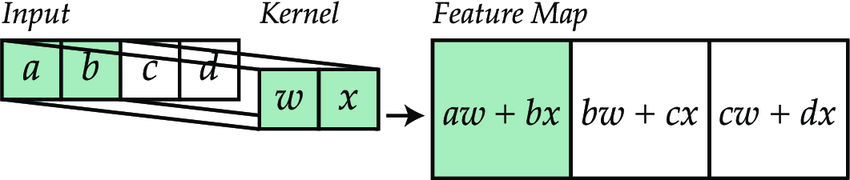
\includegraphics[width=\linewidth]{images/1d_kernel.png}
  \caption{Example of a 1D kernel (taken from \cite{1dkernel})}
  \label{fig:1dkernel}
\end{figure}
\FloatBarrier

\subsection{2D CNN}
Two-dimensional CNNs are composed of 2D kernels that will operate on multiple channels at the same time. This means that we give as input a tensor of dimensions \((N, C, H, W)\), with \(H\) the number of channels and \(W\) the length of each signal. The use of \(H\) and \(W\) as dimensions is not an arbitrary choice. Indeed, we can think of this superposition of channels as a picture, where each signal is a position on the \(y\)-axis and every timepoint a position on the \(x\)-axis. Here, \(C=1\) as this virtual picture is simply represented by nuances of grey.

\subsection{Results}
Both type of CNN works well.

\section{Discussion}
\label{sec:discussion}

\section{Conclusion}
\label{sec:conclusion}


%%%%%%%%%% ETHICAL RISKS %%%%%%%%%%
%% 200 to 400 words max., does not count in the 4-page limit
\section{Ethical risks}
It is clear that the analysis of EEG and other brain signals present a unique set of ethical challenges. Firstly, EEG signals reveal information not only about the physical health of a subject, but also mental states, emotions and cognitive functions. Acquiring and analysing EEG data requires privacy and anonymization measures to avoid unauthorized surveillance and discrimination. For example, EEG signals can now be used to identify and authenticate users based on their brain activity. However, the privacy implications of such tools remain an open question, as highlighted in \cite{eeg_authentication}.

A second ethical question comes directly from the algorithms themselves: Machine Learning tools are known to be prone to biases, especially when datasets lack diversity. This lack of inclusivity reduces the accuracy of algorithms for underrepresented groups, potentially leading to unequal outcomes in medical or cognitive assessments. Ensuring diversity in training data particularly important for clinical tools that rely on the analysis of brain activity.

The collection of EEG data is not exempt from ethical dilemmas. For instance, Neuralink’s announcement of a successful implantation of the world’s first "brain-reading device" in a human sparked controversy. The study lacked adherence to established principles of scientific ethics, particularly in providing clear information to participants and transparency to the research community, as the study was not listed on the online repository, and its protocol not disclosed. It is critical that users and subjects can give their informed consent. It is critical that users and participants must fully understand the potential risks and implications of their involvement to give an informed consent. In the data used in this project, the sEEG electrodes were already implanted in every participants, so no invasive surgery nor operations was needed.

The access to EEG-based technologies also raises issues. The high costs and complexity of these tools could limit their availabilities to poorer populations. Without efforts, this situation will exacerbate the existing disparities in healthcare.

Overall, on top of the ethical considerations specific to ML applications such as data privacy and algorithmic fitness, EEG-based tools need to address equity, user consents and usage risks. These challenges must be addressed to advance towards responsible and clinical-forward tools.

%% Not in the 4-page limit
\section{Appendix}

\begin{figure}[h!]
    \center
    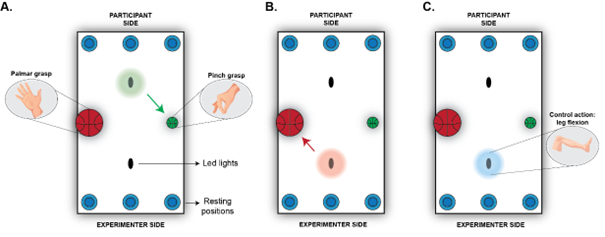
\includegraphics[width=\linewidth]{images/2024-12-11-13-41-23.png}
    \caption{Experimental setup}
\end{figure}
\FloatBarrier


% \begin{figure}[tbp]
%   \centering
%   \includegraphics[width=\columnwidth]{denoised_signal_1d}
%   \caption{Signal compression and denoising using the Fourier basis.}
%   \vspace{-3mm}
%   \label{fig:denoise-fourier}
% \end{figure}


\section*{Acknowledgements}
We thank Leonardo Pollina for taking us with him on this project, and for his quick and helpful answers to all our questions.

\bibliographystyle{IEEEtran}
\bibliography{ref}

\end{document}

% <a href="https://www.vecteezy.com/free-vector/brain-diagram">Brain Diagram Vectors by Vecteezy</a>